\documentclass[conference]{IEEEtran}
\IEEEoverridecommandlockouts
% The preceding line is only needed to identify funding in the first footnote. If that is unneeded, please comment it out.
\usepackage{cite}
\usepackage{amsmath,amssymb,amsfonts}
\usepackage{textcomp}
\usepackage{xcolor}
\usepackage{url}
\usepackage{enumerate}
\usepackage{makecell}
\usepackage{listings}
\usepackage{wrapfig}
\usepackage{paralist}
\usepackage{xspace}
\usepackage{color}
\usepackage{times}
\usepackage{proof}
\usepackage{algorithm}
\usepackage[noend]{algpseudocode}
\usepackage{capt-of}
\usepackage{enumitem}
\usepackage[pdftex]{graphicx}
\usepackage{epstopdf}
\usepackage{diagbox}
\usepackage{multirow}
\usepackage{hyperref}
\usepackage{stfloats}

%%


%Transition system
\newcommand{\TS}[1]{\ensuremath{\mathcal{T}_{#1}}}
\newcommand{\states}[1]{\ensuremath{\mathcal{C}_{#1}}}
\newcommand{\transitions}[1]{\ensuremath{\mathcal{R}_{#1}}}
\newcommand{\transition}[1]{\ensuremath{\mathit{t}_{#1}}}
\newcommand{\labels}[1]{\ensuremath{\Sigma_{#1}}}
\newcommand{\enable}[1]{\ensuremath{\mathit{en}_{#1}}}
\newcommand{\reachstates}[1]{\ensuremath{\mathit{RS}_{#1}}}

\newcommand{\location}[1]{\ensuremath{\mathit{L}_{#1}}}
\newcommand{\regionstructure}[1]{\ensuremath{\mathcal{S}_{#1}}}
\newcommand{\regions}[1]{\ensuremath{\mathcal{Q}_{#1}}}

%\newcommand{\AP}{\mathit{AP}}

\newcommand{\reaches}{\ensuremath{\leadsto}}

% BIP
\newcommand{\BIP}{\ensuremath{\textsc{BIP}}\xspace}
\newcommand{\bipvar}[1]{\ensuremath{\mathbb{V}_{#1}}}
\newcommand{\varstate}[1]{\ensuremath{\mathbf{V}_{#1}}}
\newcommand{\locs}[1]{\ensuremath{\mathbb{L}_{#1}}}
\newcommand{\locerr}[1]{\ensuremath{\mathbb{L}_{err_{#1}}}}
\newcommand{\ports}[1]{\ensuremath{\mathbb{P}_{#1}}}
\newcommand{\edges}[1]{\ensuremath{\mathbb{E}_{#1}}}
\newcommand{\init}[1]{\ensuremath{\mathbb{I}_{#1}}}
\newcommand{\allports}{\ensuremath{\bigcup_{i = 1}^n{\ports{i}}}}
\newcommand{\bexp}[1]{\ensuremath{\mathcal{F}_{#1}}}
\newcommand{\expr}[1]{\ensuremath{\mathcal{E}_{#1}}}
\newcommand{\compstate}[1]{\ensuremath{\langle l_{#1}, \mathbf{V}_{#1} \rangle}}
\newcommand{\components}{\ensuremath{\mathcal{B}}}
\newcommand{\bipmodel}{\ensuremath{\mathcal{M}_{\BIP}}}
\newcommand{\comp}[1]{\ensuremath{B_{#1}}}
\newcommand{\region}[1]{\ensuremath{\langle l_{#1}, \phi_{#1} \rangle }}
\newcommand{\portid}[1]{{\ensuremath{id({#1})}}}

\newcommand{\variable}[1]{\ensuremath{\mathbb{V}_{#1}}}



%ART
%\newcommand{\region}[1]{\ensuremath{\psi_{#1}}}
\newcommand{\ART}[1]{\ensuremath{\mathbb{T}_{#1}}}
\newcommand{\artnode}[1]{\ensuremath{\mathit{nd}_{#1}}}
\newcommand{\artroot}{\ensuremath{\mathit{Root}}}
\newcommand{\nodes}{\ensuremath{\mathit{Nodes}}}
\newcommand{\artedge}{\ensuremath{\mathit{Edges}}}
\newcommand{\covers}{\ensuremath{\mathit{Covers}}}
\newcommand{\artpath}{\ensuremath{\pi}}
\newcommand{\interpolant}[1]{\ensuremath{\mathbf{I}_{#1}}}
\newcommand{\cex}[1]{\ensuremath{\mathit{cex}_{#1}}}
\newcommand{\leafs}{\ensuremath{\mathit{Leafs}}}


% POR
\newcommand{\enabled}{\ensuremath{\Gamma_{enab}}}
\newcommand{\sset}{\ensuremath{\Gamma_{sim}}}
\newcommand{\pset}{\ensuremath{\Gamma_{per}}}
\newcommand{\aset}{\ensuremath{\Gamma_{amp}}}
\newcommand{\sbset}{\ensuremath{\Gamma_{stub}}}

%
% Useful symbols and abbreviations
%
\newcommand{\Nat}{\mathbb{N}}    % natural numbers
\newcommand{\Real}{\mathbb{R}}   % real numbers
\newcommand{\Int}{\mathbb{Z}}    % integers
\newcommand{\xone}[2]{#1_1,\ldots,#1_{#2}}   % variable range from 1
\newcommand{\xzero}[2]{#1_0,\ldots,#1_{#2}}  % variable range from 0
\newcommand{\CalC}{\mathcal{C}}              % example of caliph C
\newcommand{\setof}[1]{\{#1\}}               % set
\newcommand{\powerset}[1]{2^{#1}}   % power set
\newcommand{\Def}{\stackrel{\mathrm{def}}{=}}   % definition
\newcommand{\mktuple}[1]{\ensuremath{\langle{#1}\rangle}} % tuple definition
\newcommand{\true}{\ensuremath{\mathit{true}}}
\newcommand{\false}{\ensuremath{\mathit{false}}}


% Software model checkers and tools.
\newcommand{\kratos}{\textsc{Kratos}\xspace}
\newcommand{\nusmv}{\textsc{NuSMV}\xspace}
\newcommand{\nuxmv}{\textsc{nuXmv}\xspace}
\newcommand{\mathsat}{\textsc{MathSAT}\xspace}
\newcommand{\dfinder}{\textsc{DFinder}\xspace}
\newcommand{\vcs}{\textsc{VCS}\xspace}


\newtheorem{definition}{Definition}

\setlength{\textfloatsep}{5pt}

\newcommand{\tabincell}[2]{\begin{tabular}{@{}#1@{}}#2\end{tabular}}

\hypersetup{
	colorlinks=true,
	linkcolor=blue,
	filecolor=blue,
	urlcolor=blue,
	citecolor=cyan,
}

\def\BibTeX{{\rm B\kern-.05em{\sc i\kern-.025em b}\kern-.08em
    T\kern-.1667em\lower.7ex\hbox{E}\kern-.125emX}}
\begin{document}

\title{Behavioral fault modeling and analysis with BIP:\\
	A Wheel Brake System Case Study\\}

\author{\IEEEauthorblockN{1\textsuperscript{st} Xudong Tang}
\IEEEauthorblockA{\textit{Shanghai Key Lab for Trustworthy Computing} \\
\textit{East China Normal University }\\
Shanghai, China \\
51184501045@stu.ecnu.edu.cn}
\and
\IEEEauthorblockN{2\textsuperscript{nd} Qiang Wang}
\IEEEauthorblockA{\textit{dept. name of organization (of Aff.)} \\
\textit{name of organization (of Aff.)}\\
City, Country \\
email address or ORCID}
\and
\IEEEauthorblockN{3\textsuperscript{rd} Weikai Miao}
\IEEEauthorblockA{\textit{dept. name of organization (of Aff.)} \\
\textit{name of organization (of Aff.)}\\
Shanghai, China \\
wkmiao@sei.ecnu.edu.cn}
}

\maketitle

\begin{abstract}
BIP(Behavior-Interaction-Priority) is a component-based framework for rigorous design of complex systems. Systems are modeled by a set of components and connectors.
Behavioral fault modeling and analysis refers to an integration of model based system design and safety analysis. In this paper, we integrate fault tree based safety analysis into BIP model and apply statistical model checking to verify system specification and calculate probability of fault issues. We also trace the simulation result to confirm the extended system model without fault keeps consistence of the norminal system model.  
We illustrate an airplane wheel brake system meeting the industry standards as case study to show its advantage in analyzing fault behavior of safety-critical systems in aerospace practice.
\end{abstract}

\begin{IEEEkeywords}
model checking, safety analysis, fault tree, BIP
\end{IEEEkeywords}

\section{Introduction}
\textcolor{red}{
Giving introduction of BIP framework, BIP toolset, SBIP and, on the other hand, faulttree-based safety analysis. Using structure of the paper as ending.
}

\section{Preliminaries}

\subsection{The BIP Framework}
We use architecture diagrams \cite{} to model the architecture styles in BIP.
An architecture diagram consists of a set of component types, with associated cardinality constraints representing the
expected number of instances of each component type and a set of connector motifs.
Connector motifs, which define sets of BIP connectors, are non-empty sets of port types, each labelled as either a trigger or a synchron.
Each port type has a cardinality constraint representing the expected number of port instances
per component instance and two additional constraints: multiplicity and degree,
represented as a pair m : d. Multiplicity constrains the number of instances of
the port type that must participate in a connector defined by the motif; degree
constrains the number of connectors attached to any instance of the port type.

In this section, we present the BIP model with multiparty synchronization and data transfer.A BIP model is a parallel composition of a set of components.
A BIP component is formally defined as an automaton extended with linear integer arithmetic as follows.

\begin{definition} [BIP component]
	\label{component-def}
	Given a finite set of variables $\bipvar{}$, a BIP component is defined as a tuple
	$\comp{} = \mktuple{\bipvar{}, \locs{}, \ports{}, \edges{}, \ell}$, where
	\begin{inparaenum}
		\item $\locs{}$ is a finite set of control locations;
		\item $\ports{}$ is a finite set of communication ports;
		\item $\edges{} \subseteq \locs{} \times \ports{} \times \bexp{\bipvar{}} \times \expr{\bipvar{}} \times \locs{}$
		is a finite set of transition edges extended with guards in $\bexp{\bipvar{}}$
		and operations in $\expr{\bipvar{}}$;
		\item $\ell \in \locs{}$ is an initial control location.
	\end{inparaenum}
\end{definition}

Transition edges in a component are labeled by ports, which form the interface of the component.
We assume that, from each control location,
every pair of outgoing transitions have different ports,
and the ports of different components are disjoint.
In other words, transitions with the same ports in the component are not enabled simultaneously.
Given a component violating such assumptions,
one can easily transform it into the required form by renaming the ports,
while retaining the BIP expressiveness power.
To ease the presentation, we denote in the sequel the id of the unique component
where port $p$ is defined by $\portid{p}$.

%Given a tuple of component types $\overline{\comptype{}} = \mktuple{\comptype{1},\ldots, \comptype{k}}$,
%and a tuple of natural numbers $\overline{n} = \mktuple{n_{1}, \ldots, n_{k}}$,
%where $n_{i}$ represents the number of instantiations of $\comptype{i}$,
%

We denote by $\components = \{\comp{i} ~|~ i\in [1,n]\}$ a set of components.
%instantiated from $\overline{\comptype{}}$.
%where $\comptype{i}[j]$
%$\comptype{i}[j] = \mktuple{\bipvar{i}[j] ,\locs{i}[j] ,\ports{i}[j], \edges{i}[j], \ell_{i}[j] }$
%is the $j^{th}$ instantiation of component type $\comptype{i}$.
%
%Given a set of comoponents $\components$,
In \BIP, coordinations of components are specified by using interactions.
%and in \BIP an interaction is represented as a finite set of ports.

\begin{definition} [Interaction]
	\label{interaction}
	An interaction for $\components $ is a tuple $\gamma = \mktuple{g, \mathcal{P}, f } $,
	where $g \in \bexp{\bipvar{}}$, $f\in \expr{\bipvar{}}$ and
	$\mathcal{P} \subseteq \bigcup_{i=1}^n \ports{i}$, $\mathcal{P} \neq \emptyset$, and
	for all $i \in [1, n]$, $|\mathcal{P} \cap \ports{i}| \le 1$.
\end{definition}

Intuitively, an interaction defines a guarded multiparty synchronization with data transfer:
when the guard $g$ of an interaction $\mathcal{P}$ is enabled,
then the data transfer specified by $f$ can be executed, and
after that the transitions labelled by the ports in $\gamma$ can be taken simultaneously.
%
We denote by $\Gamma$ a finite set of interactions.
A \BIP model is constructed by composing a number of components with interactions.

\begin{definition} [\BIP Model]
	A \BIP model $\bipmodel$ is a tuple $\mktuple{\components,\Gamma}$,
	where $\components$ is a finite set of components,
	and $\Gamma$ is a finite set of interactions for $\components$.
\end{definition}

We do not take priority into account in this paper, as in the previous work~\cite{dfinder10,tgc15},
since adding priority will not introduce any errors.
If a model without priority is safe, then after adding priority constraints it remains safe.
We use a simple mutual exclusion protocol to illustrate \BIP.

%\input{ticket-bip}

A state of a \BIP model is a tuple $c = \langle \compstate{1}, \ldots, \compstate{n} \rangle $,
where for all $i \in [1,n] $, $l_i \in \locs{i} $ and $\mathbf{V}_i $ is a valuation of $\bipvar{i}$.
%
%We denote by $c(i,j), i\in[1,k]$ the state $\mktuple{l_{i}^{j}, s_{i}^{j}}$ of component $\comptype{i}[j]$.
%$c_0=\mktuple{\mktuple{l_1,s_1},\ldots, \ldots, \mktuple{l_n,s_n}}$
A state $c_{0}$ is initial if for all $i \in [1,n]$,
$l_i = \ell_{i}$ and $\mathbf{V}_{i}$ is the initial valuation of $\bipvar{i}$.
%
A state $c$ is an error if for some $i \in [1,n]$, $l_{i}$ is an error location.
%
We say an interaction $\gamma \in \Gamma$ is enabled on a state $c$ if
for every component $\comp{i} \in \components$,
such that $\gamma \cap \ports{i} \neq \emptyset$,
%
there is an edge $\mktuple{l_i, \gamma \cap \ports{i}, g_i, f_i, l_{i}' } \in \edges{i}$
and  $\mathbf{V}_{i} \models g_i $.
%
The labeled transition system semantics of a \BIP model is defined as follows.

\begin{definition} [\BIP operational semantics]
	\label{operational-semantics}
	Given a \BIP model $\bipmodel=\mktuple{\components,\Gamma}$,
	its operational semantics is defined by a labeled transition system
	$\TS{\BIP} = \mktuple{\mathcal{C}, \Sigma, \mathcal{R}, \mathcal{C}_{0}}$, where
	%
	\begin{enumerate}
		\item $\mathcal{C}$ is the set of states,
		\item $\Sigma = \Gamma $,
		\item $\mathcal{R}$ is the set of transitions,
		and we say that there is a transition from a state $c$
		%$c=\mktuple{\mktuple{l_1,s_1}, \ldots, \mktuple{l_n,s_n}} $
		to another state $c'$,
		%$c'=\mktuple{\mktuple{l_1',s_1'}, \ldots, \mktuple{l_n',s_n'}}$
		if there is an interaction $\gamma $ such that,
		%
		\begin{enumerate}
			%\begin{inparaenum}[(i)]
			\item $\gamma$ is enabled in $c$;
			\item for all $\comp{i} \in \mathbb{B}$ such that
			$\gamma \cap \ports{i} \neq \emptyset$, there is an edge
			$\mktuple{l_i, \gamma \cap \ports{i}, g_i, f_i, l_i'} \in \edges{i} $,
			%and if $f_i = x := e $,
			then $\mathbf{V}'_{i} = \mathbf{V}_{i}[\bipvar{} / f_i(\bipvar{})]$;
			\item for all $\comp{i} \in \mathbb{B} $ such that
			$\gamma \cap \ports{i} = \emptyset $,
			$l_i' = l_i$ and $\mathbf{V}_i' = \mathbf{V}_i$.
			%\end{inparaenum}
		\end{enumerate}
		\item $\mathcal{C}_{0}$ is the set of initial states.
	\end{enumerate}
\end{definition}

%We denote by $c \overset{\gamma} \rightarrow c'$ that
%there is a transition from state $c$ to state $c'$, following the interaction $\gamma$.
%
%We denote by $\rho$
%
%A state $c$ % $c=\mktuple{\mktuple{l_1,s_1}, \ldots, \mktuple{l_n,s_n}}$
%is reachable if there is a trace
%$c_0, c_1, \ldots, c_k$ such that
%$c_0 \xrightarrow{\gamma_1} c_1 \xrightarrow{\gamma_2} \ldots \xrightarrow{\gamma_k} c $,
%from an initial configuration $c_{0}$ to $ c$.
%

\subsection{Statistical Model Checking}
\textcolor{red}{
Giving an introduction of Statistical Model Checking here.
}

\section{The AIR6110 Wheel Brake System}
The Wheel Brake System(WBS) description is introducted in Aerospace Information Report 6110(AIR6110)[] as a contiguous aircraft system development process example. According to AIR6110 standard, WBS is a detailed funciton of an aircraft designated model S18. The hypothetical S18 aircraft is a two engine passenger aircraft designed to carry 300 to 350 passengers up to 5000 nautical miles at
0.84 mach, and has an average flight duration of 5 hours. 

The WBS provides braking on the main gear wheels used to provide safe retardation of the aircraft during taxiing and landing phases, and in the event of a rejected take-off. The wheel brakes also prevent unintended aircraft motion when parked, and may be used to provide differential braking for aircraft directional control. A secondary function of the WBS is to stop main gear wheel rotation upon gear retraction. Braking on the ground is commanded manually, via brake pedals, or automatically (autobrake) without the need for pedal application.

\begin{figure}[htbp]
	\centerline{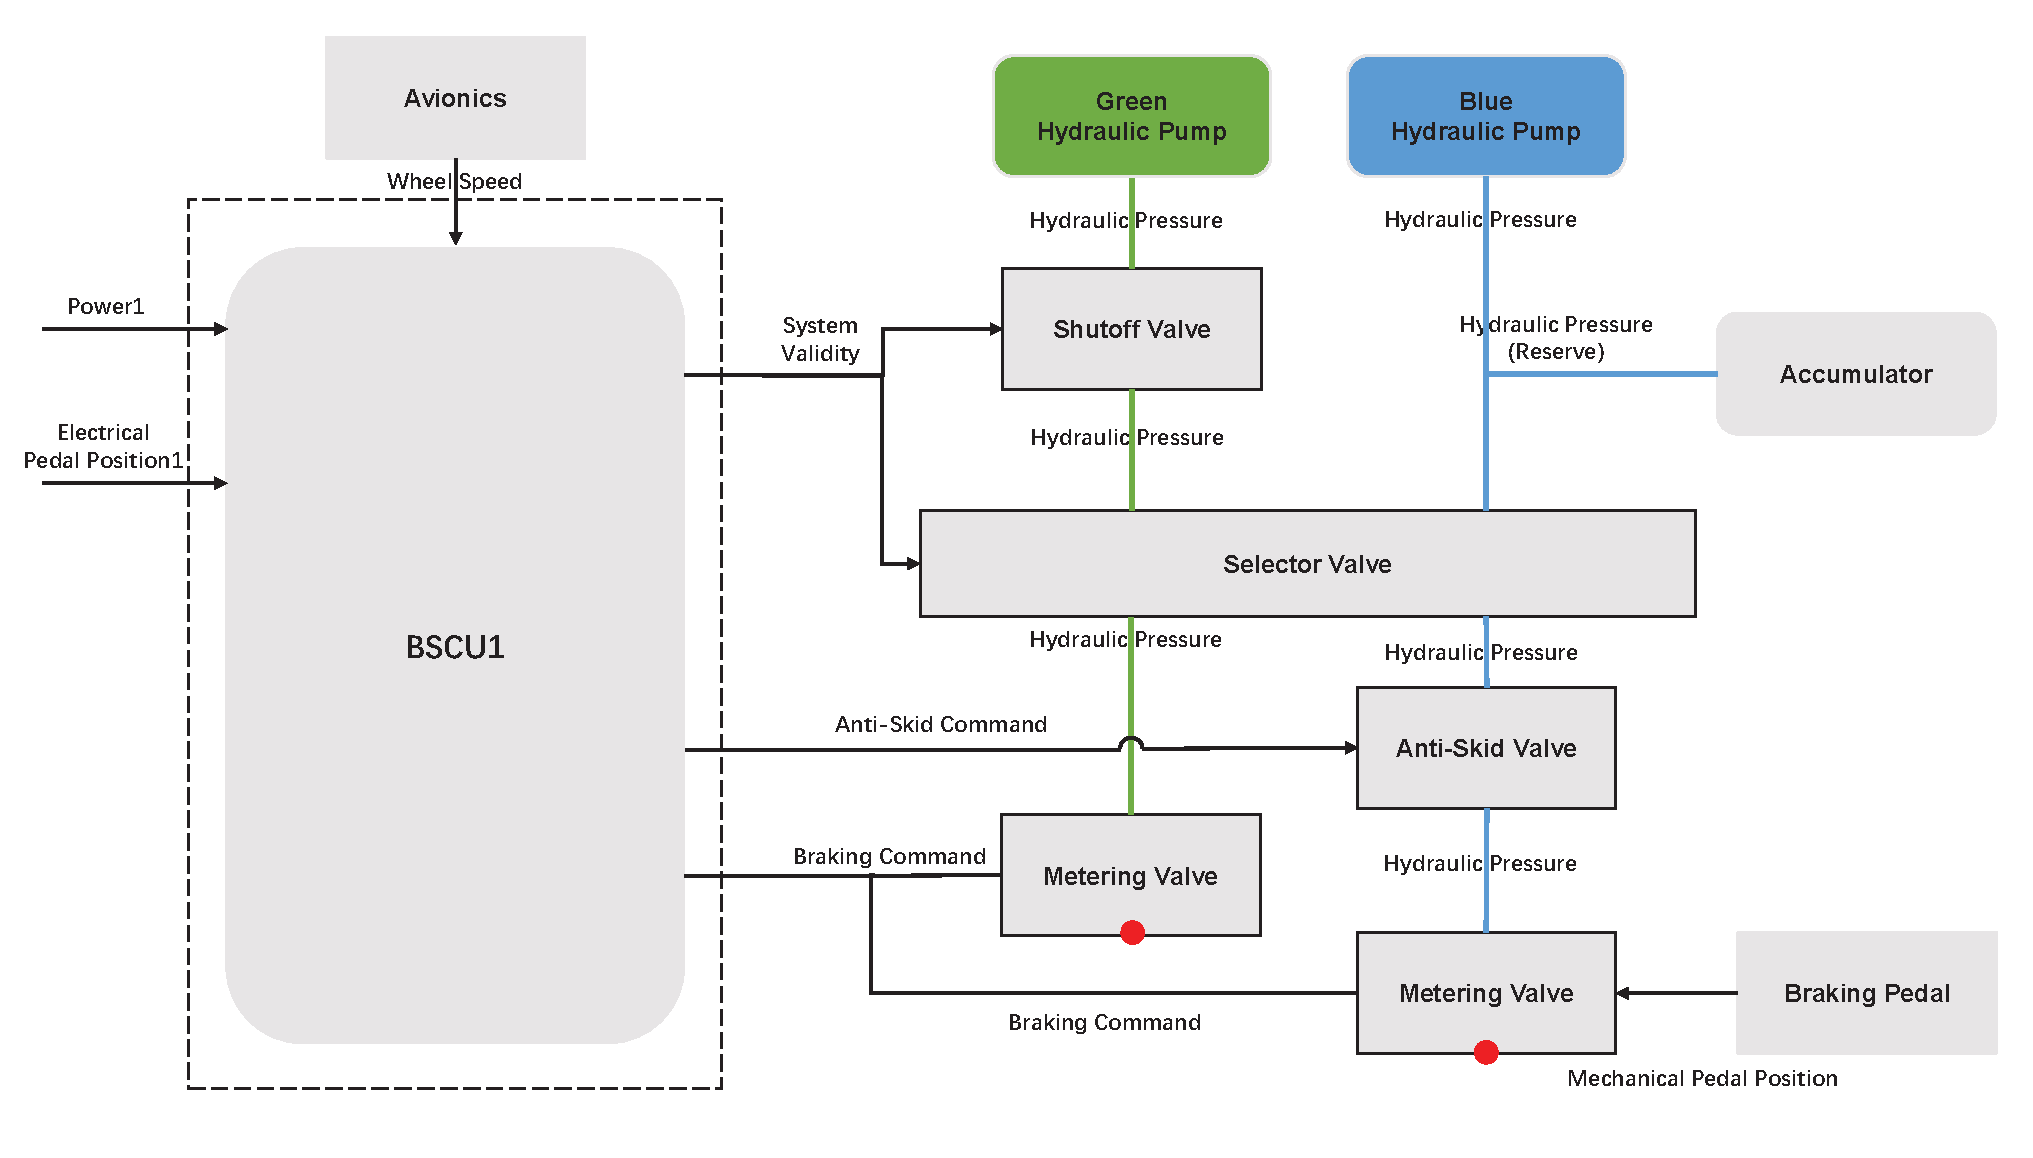
\includegraphics[width=85mm]{figure/Nominal.eps}}
	\caption{The WBS BIP model of the nominal behavior}
	\label{WBS_BIP_Nominal}
\end{figure}

\subsection{The WBS architecture and nominal behavior}
Figure 1 shows the WBS BIP model of the nominal behavior. The WBS is composed of an electronic control system and a physical system. The majority of the electronic control system is Braking System Control Unit(BSCU). The WBS receives several signals including the brake pedal position from upper level avionics system and electically forwards them to the BSCU. The BSCU also receives two power inputs from two independent power supply resources. As the result of computation, the BSCU in turn produces the system validity command, anti-skid command and braking command to the physical system. The physical system includes two hydraulic pressure lines which are supplied by the green/blue hydraulic pump respectively.

\emph{Operation Mode.} There are three operation modes for physical system. In \emph{normal mode}, the wheel brake is supported by the main hydraulic circuit, refers to the green hydraulic circuit. In \emph{alternate mode}, the wheel brake is supported by a second hydraulic circuit. This mode is standby and is selected automatically when the normal system fails. An accumulator supplies the \emph{emergency mode} when blue hydraulic supply is lost and the normal mode is not available.

\emph{Braking System Control Unit(BSCU).} According to the AIR6110 standard, for redundancy, the BSCU is composed of two independent channels, each channel has its own power supply and avioncs system inputs. Each channel has a command subsystem and a monitor subsystem. The monitor system generates the system validity command and the command system cauculates the anti-skid command and braking command. The BSCU will make an ultimate judgement call between each command output by the two channels respectively.

\emph{Hydraulic Pump.} In nominal system behavior, both the green and blue hydraulic pumps provide enough hydraulic pressure for their green/blue hydraulic circuit respectively. An accumulator is also a hydraulic pump to provide an emergency reserve of hydraulic pressure for blue hydraulic circuit in emergency mode.

\emph{Shutoff Valve.} The shutoff valve responds the system validity command from BSCU to decide whether to apply the hydraulic pressure to the selector valve in green hydraulic circuit or not. The system validity command is modeled in BIP as a boolean value.

\emph{Selector Valve.} The selector valve control the switch between green and blue hydraulic circuits mechanically. It outputs appropriate pressure from green hydraulic pump, and switches to blue hydraulic circuit as soon as it detects a lack of pressure in the green hydraulic circuit. In BIP model, the component selector valve 
only outputs pressure from either the green hydraulic circuit input or blue hydraulic circuit input at a time.

\emph{Anti-Skid Valve.} The anti-skid valve follows anti-skid command to control hydraulic pressure to the metering valve. It is used to restrict the hydraulic pressure to the wheel brake in order to prevent locking of the wheel. Wheel skid happens when the wheel is locked but the vehicle keeps a relative slid speed to the ground. We consider a loss of anti-skid function as a fault and will integrate it into nominal BIP model.

\emph{Metering Valve.} Metering valve, or metering servo valve controls pressure to the demanded level and provides regulation for the anti-skid function.

\subsection{The WBS architecture mode in BIP}
According to the AIR6110 standard, the system architecture evolves throughout the development life cycle and is tightly coupled with the requirements development (especially interface requirements) and is not finished until the requirements associated with the architecture have been validated.

We follow the standard to advance our BIP model. As a result, our WBS BIP model has four versions corresponding to the four architectures in the AIR6110 standard. They are numbered from ARCH1 to ARCH4. Each architecture is obtained after design choices of different types.

\emph{ARCH1.} The architecture one is regarded as a high level wheel brake system architecture to be analyzed against the system level functions operational and safety requirements, and any design constraints that have been identified early in the standard.

\emph{ARCH2.} Modified braking system architecture ARCH2 implements the function of ARCH1 and meets various of derived requirements listed in the Wheel Brake System preliminary safety assessment(PSSA). As a feedback of PSSA, things to consider include but are not limited to:

\begin{itemize}
\item The modified architecture shall have at least two independent hydraulic pressure sources.
\item The modified architecture shall have dual channel BSCU and multimode brake operations to provide the required redundancy.
\end{itemize}

\emph{ARCH3.} Following the result of the WBS trade study, The development of architecture three is designed with one BSCU housing two independent systems, each BSCU subsystem has independent command and monitor channels.

\emph{ARCH4.} Since architecture three has been simulated and the results of the modeling for each system component are that the schematic of the braking system architecture does not work and there are some mistakes in the schematic. Architecture four is established to avoid the risk of hydraulic supply to wheel brake being possible in normal mode by accumulator. An input is added in ARCH4 to the selector valve corresponding to the validity of the control system. Pedal position signal is input in front of the anti-skid valve in blue hydraulic pressure line and the accumulator is moved in front of the selector valve.

\section{Integrating Fault Trees Into WBS BIP model}

\subsection{Behavioral fault modeling}
In this section, we describe how to integrate a component's fault behavior from system fault tree into the BIP model. First, we decompose the system fault tree. Then we deduce a fault behavior from each leaf node of the system fault tree. Next, we generate a BIP component with fault behavior according to its nominal behavior BIP model. Afterwards, we put the behavioral fault component and the nominal behavior component together with a manager component deciding and monitoring the activition of both fault and nominal behavior components. Finally, we modifies the connection between each component to ensure the input and output ports are the same as the original BIP component. The result of the integration is a fault-based BIP component.

\textbf{Example 1.} We take a commonly used valve component as an example. In general, a valve is used to control the passage of hydraulic pressure. When the valve is open, the output hydraulic pressure is equal to the input hydraulic pressure, indicates that the valve currently allows hydraulic pressure to pass. When the valve is close, the output hydraulic pressure is zero, indicates a rejection of hydraulic passage. We model the nominal behavior of valve in BIP, as shown in Figure 2.

\begin{figure}[htbp]
	\centerline{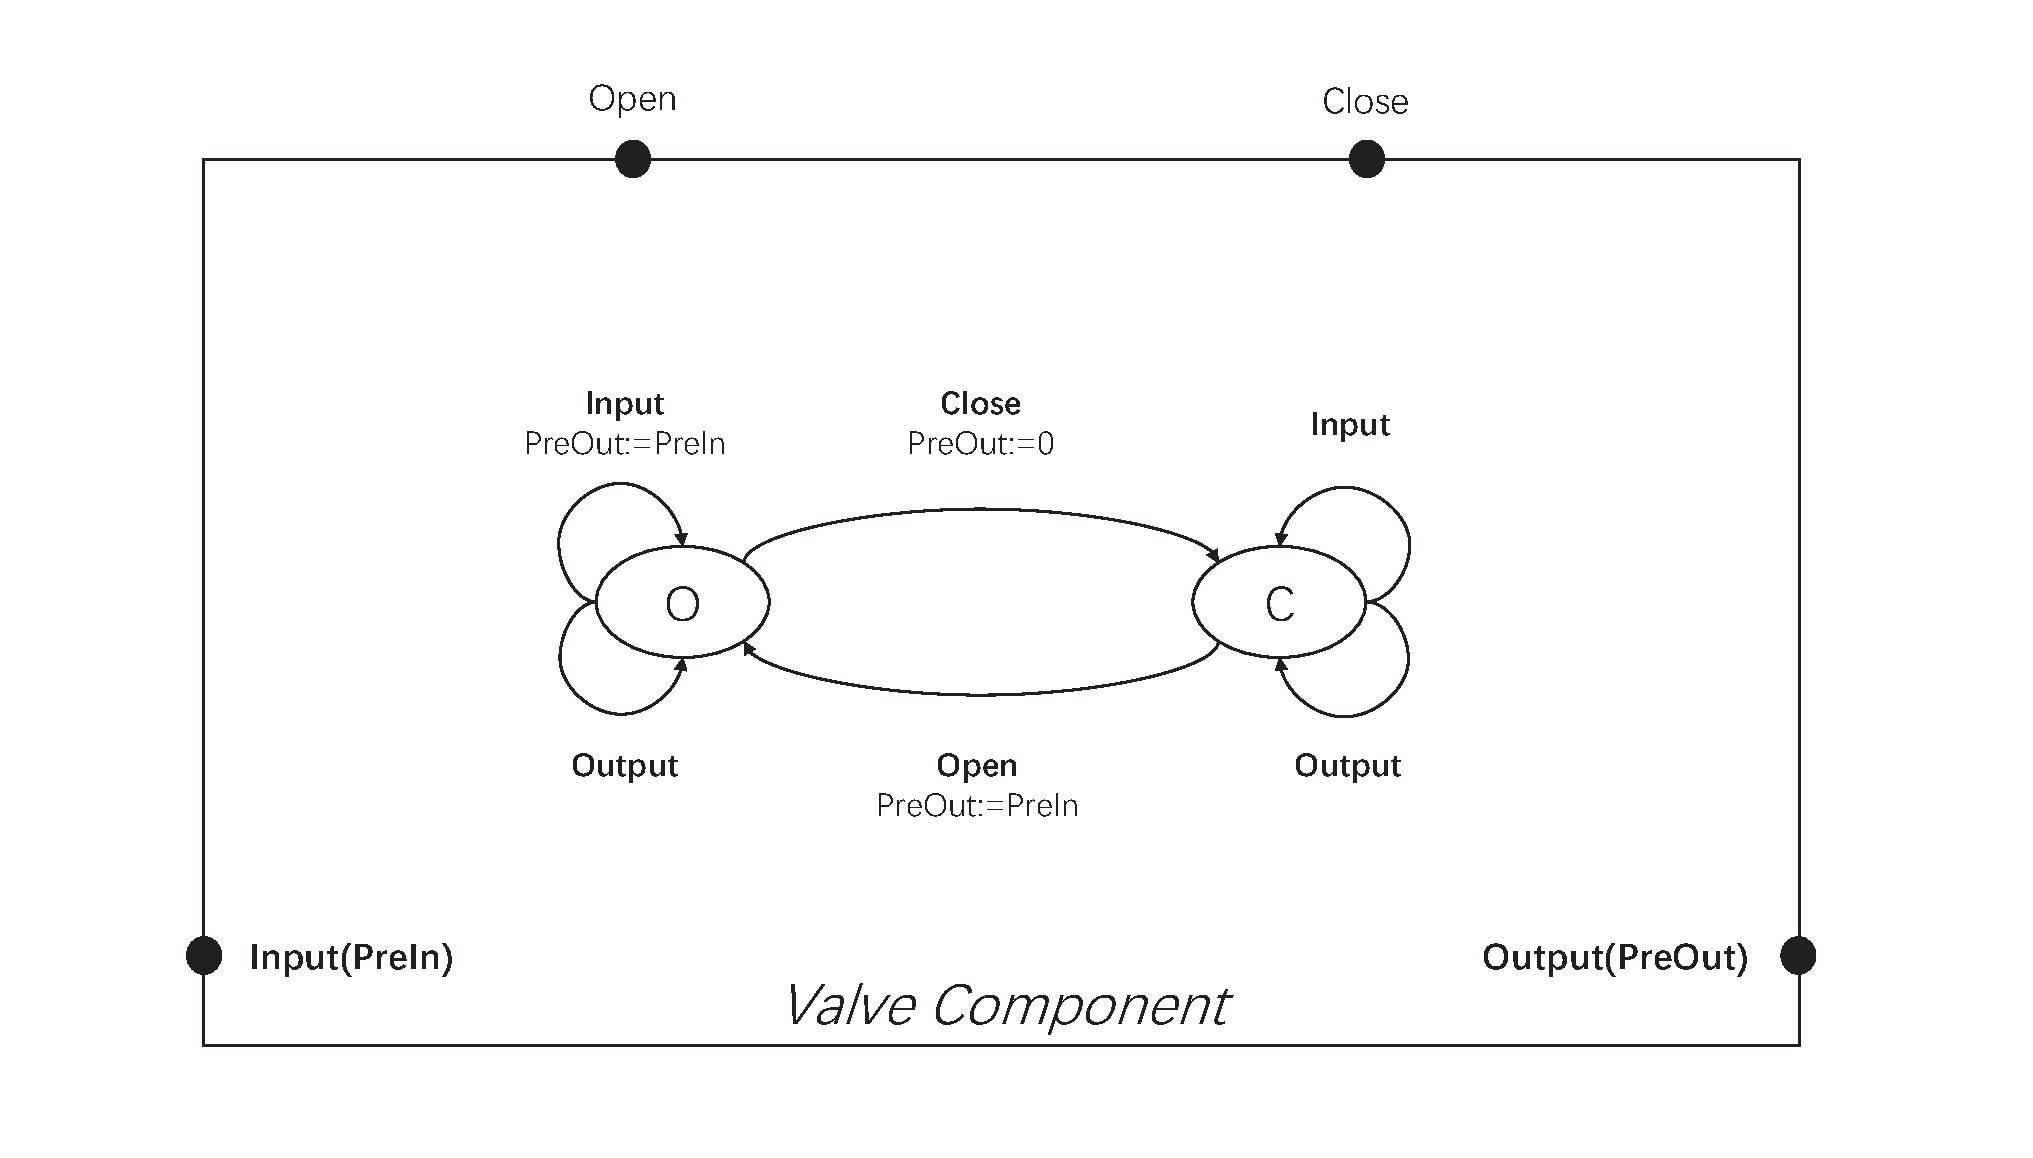
\includegraphics[width=85mm]{figure/example_origin.eps}}
	\caption{The nominal behavior of valve in BIP}
	\label{example_BIP_nominal}
\end{figure}

\begin{figure}[htbp]
	\centerline{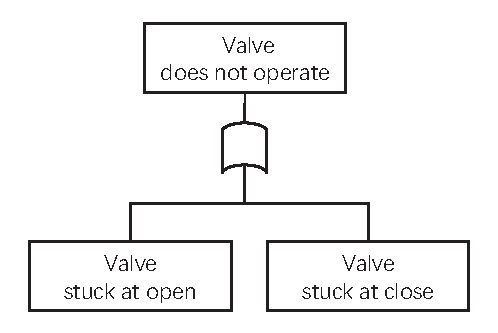
\includegraphics[width=60mm]{figure/example_fault_tree.eps}}
	\caption{Fault tree for a loss of valve occurrence}
	\label{example_BIP_nominal}
\end{figure}

Figure 3 shows the failure of valve. A loss of valve occurs when the valve is stuck at open or it is stuck at close. We deduce two fault behaviors for the valve component from the leaf nodes of this fault tree, the stack-at-open fault and stuck-at-close fault. For stuck-at-open fault, the output hydraulic pressure is always the same as the input, while for stuck-at-close fault, the output hydraulic pressure is always zero.

\emph{The integration steps.} We conclude our methodology of integrating and transforming the fault tree of figure 3 into the valve component BIP model shown in figure 2 by the following steps:

Step1: Deduce the faulty behavior from the fault tree. The top level fault, which is the loss of valve in this case, will occur through the combination of the leaf nodes with the gates. We focus on each leaf node to translate them into faulty behaviors respectively. For this case, the two leaf nodes are translated as follows:

\begin{itemize}
	\item For stuck-at-open fault, the output hydraulic pressure is always the same as the input.
	\item For stuck-at-close fault, the output hydraulic pressure is always zero.
\end{itemize}

Step2: Generate BIP component with faulty behavior. Comparing with the nominal behavior valve component, the valve with stuck at open/close fault shows an eternally unblocked/blocked for both \emph{Open} and \emph{Close} status respectively. According to step 2, the faulty behavior valve components are generated as follows:

\begin{itemize}
	\item For both faulty behavior components, the transition among \emph{Open} and \emph{Close} status will no longer change the value of \emph{PreOut}.
	\item For stuck-at-open component, the action of transition from status \emph{Close} to \emph{Close} under event \emph{Input} is \emph{PreOut:=PreIn}, just the same as transition from status \emph{Open} to \emph{Open} under event \emph{Input}.
	\item For stuck-at-close component, the action of transition from status \emph{Open} to \emph{Open} under event \emph{Input} is \emph{PreOut:=0}, just the same as transition from status \emph{Close} to \emph{Close} under event \emph{Input}.
\end{itemize}

Step3: Design a manager component for deciding and monitoring the activition of both fault and nominal behavior components. In this example, we design a manager component with three states, each of them represents one kind of valve status. Once the state execute a self circulation, an event will be sent to the corresponding behavioral component to activate it. The three states switch through internal port \emph{Trigger} which is controlled by BIP enigne to support a stochastic process of faulty behavior occured during simulation.

Step4: Since the original component has been integrated with faulty behavior, it keeps the same external port for connection  as before but has been extended a lower level to contain various of components designed in the previous steps. Modifying the upward connectors from components to the compound and extending each component with an external port receiving activation event. Confirming the extended system model without fault keeps consistence of the norminal system model through observing their transition of status, internal and external ports and connectors(This will be reconfirmed by tracing the simulation result).

As a result of integration of valve component and fault tree for loss of valve occurrence, figure 4 shows the valve compound containing a valve component with nominal behavior, two valve components with faulty behavior and a manager component. Using this BIP model, we integrate failure into the software behavior instead of separating the hardware failure from software system. As hierarchies of complex components, the integrated compound helps us observe the system behavior through graphical representation of BIP model. Also, further simulation and validation of tracing faulty behavior using stochastic BIP engine becomes possible.

\begin{figure*}[htbp]
	\centerline{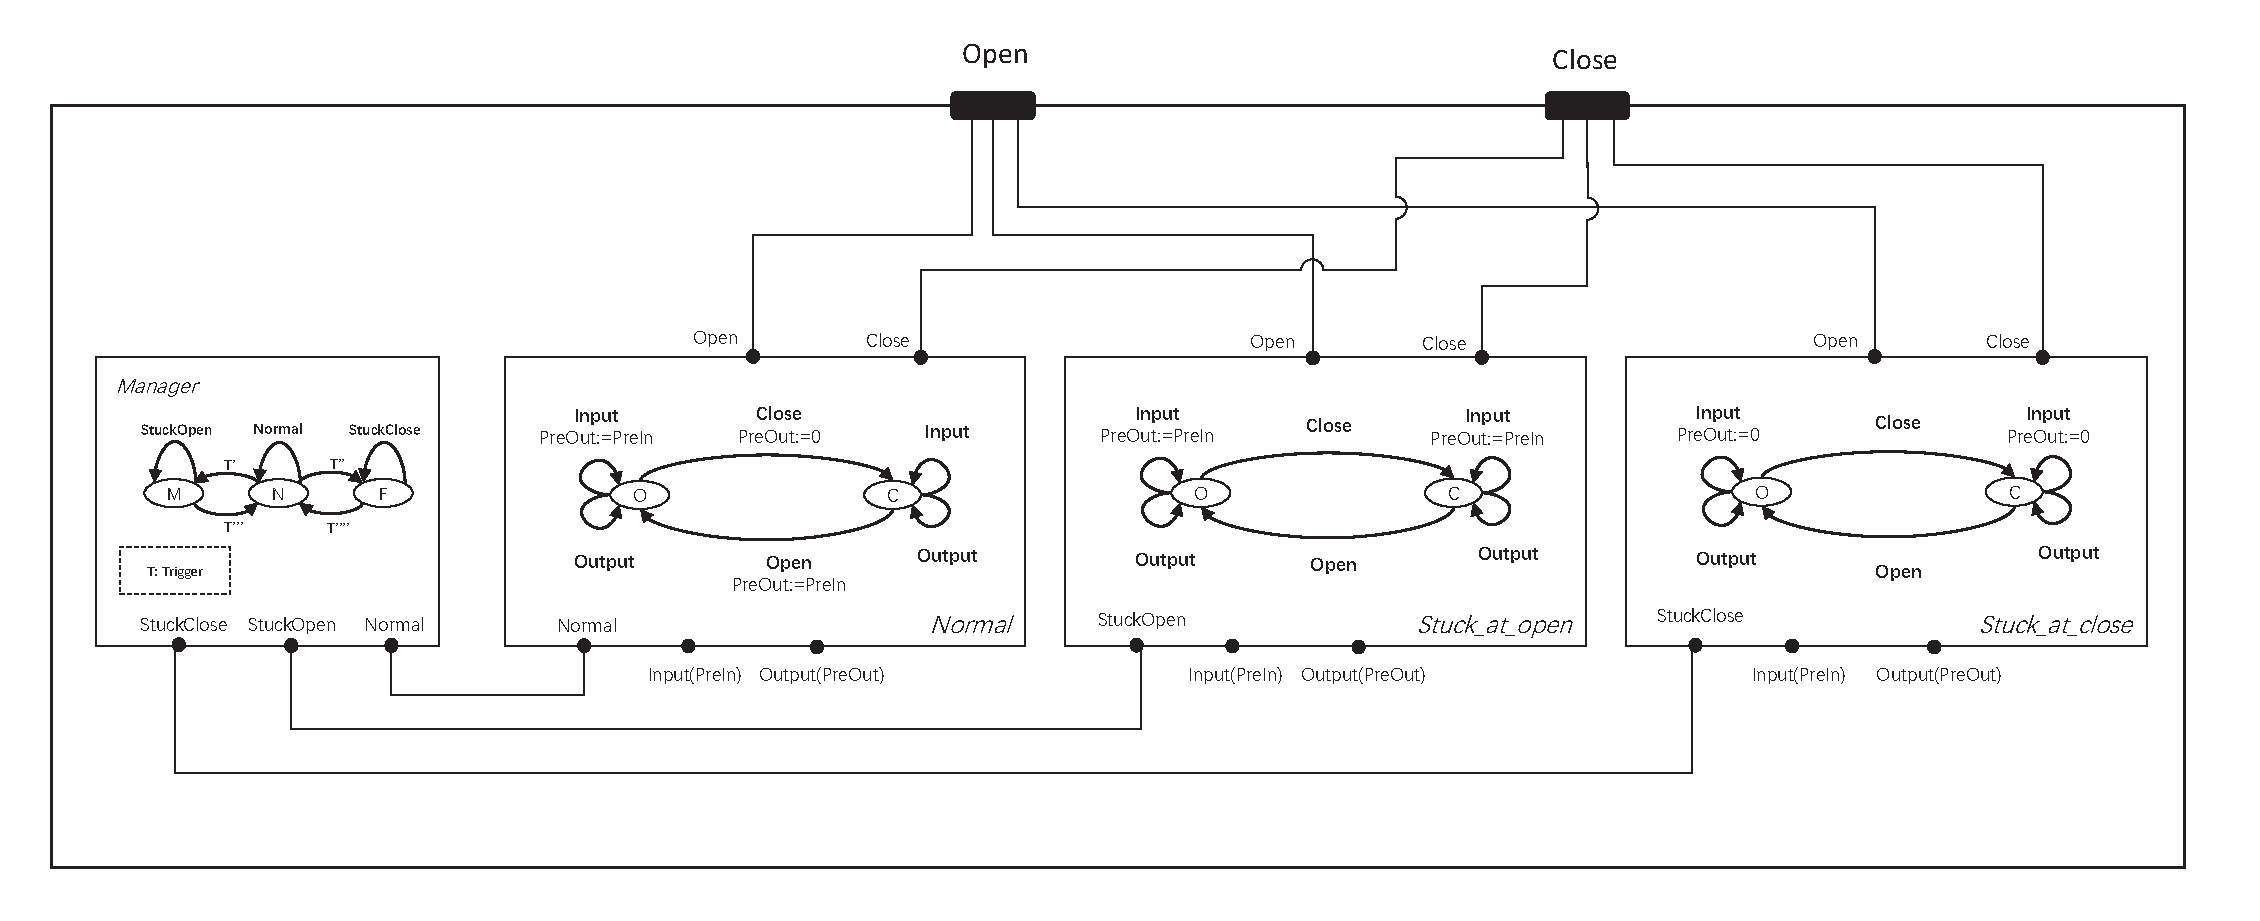
\includegraphics[width=165mm]{figure/Example.eps}}
	\caption{An integration example of common valve component}
	\label{Example}
\end{figure*}

\subsection{Fault trees for the WBS}
Figure 3 shows a fault tree for "Loss of wheel braking" event, which is based on the AIR6110 standard description. Loss of wheel braking is caused either through the Loss of operaton of physical system or due to the loss of BSCU. We focus on the leaf nodes which represent fault behavior for their component respectively. Notice that the expansion of the fault tree nodes "Loss of BSCU channel 1/2" are carried out but not included in figure 3 for the sake of brevity. 

We deduce the faulty behaviors for every component from the fault tree shown in figure 3. Also, we consider the compound \emph{BSCU Channel 1/2} as the lowest level of component for the sake of brevity. A statistics of deduced faulty behaviors is given in table 1. The selector valve's faulty behavior is loss of its selector function, while each BSCU channel has three faulty behaviors including "loss of power supply", "loss of monitor system" and "command system does not operate".

\begin{figure*}[hb]
	\centerline{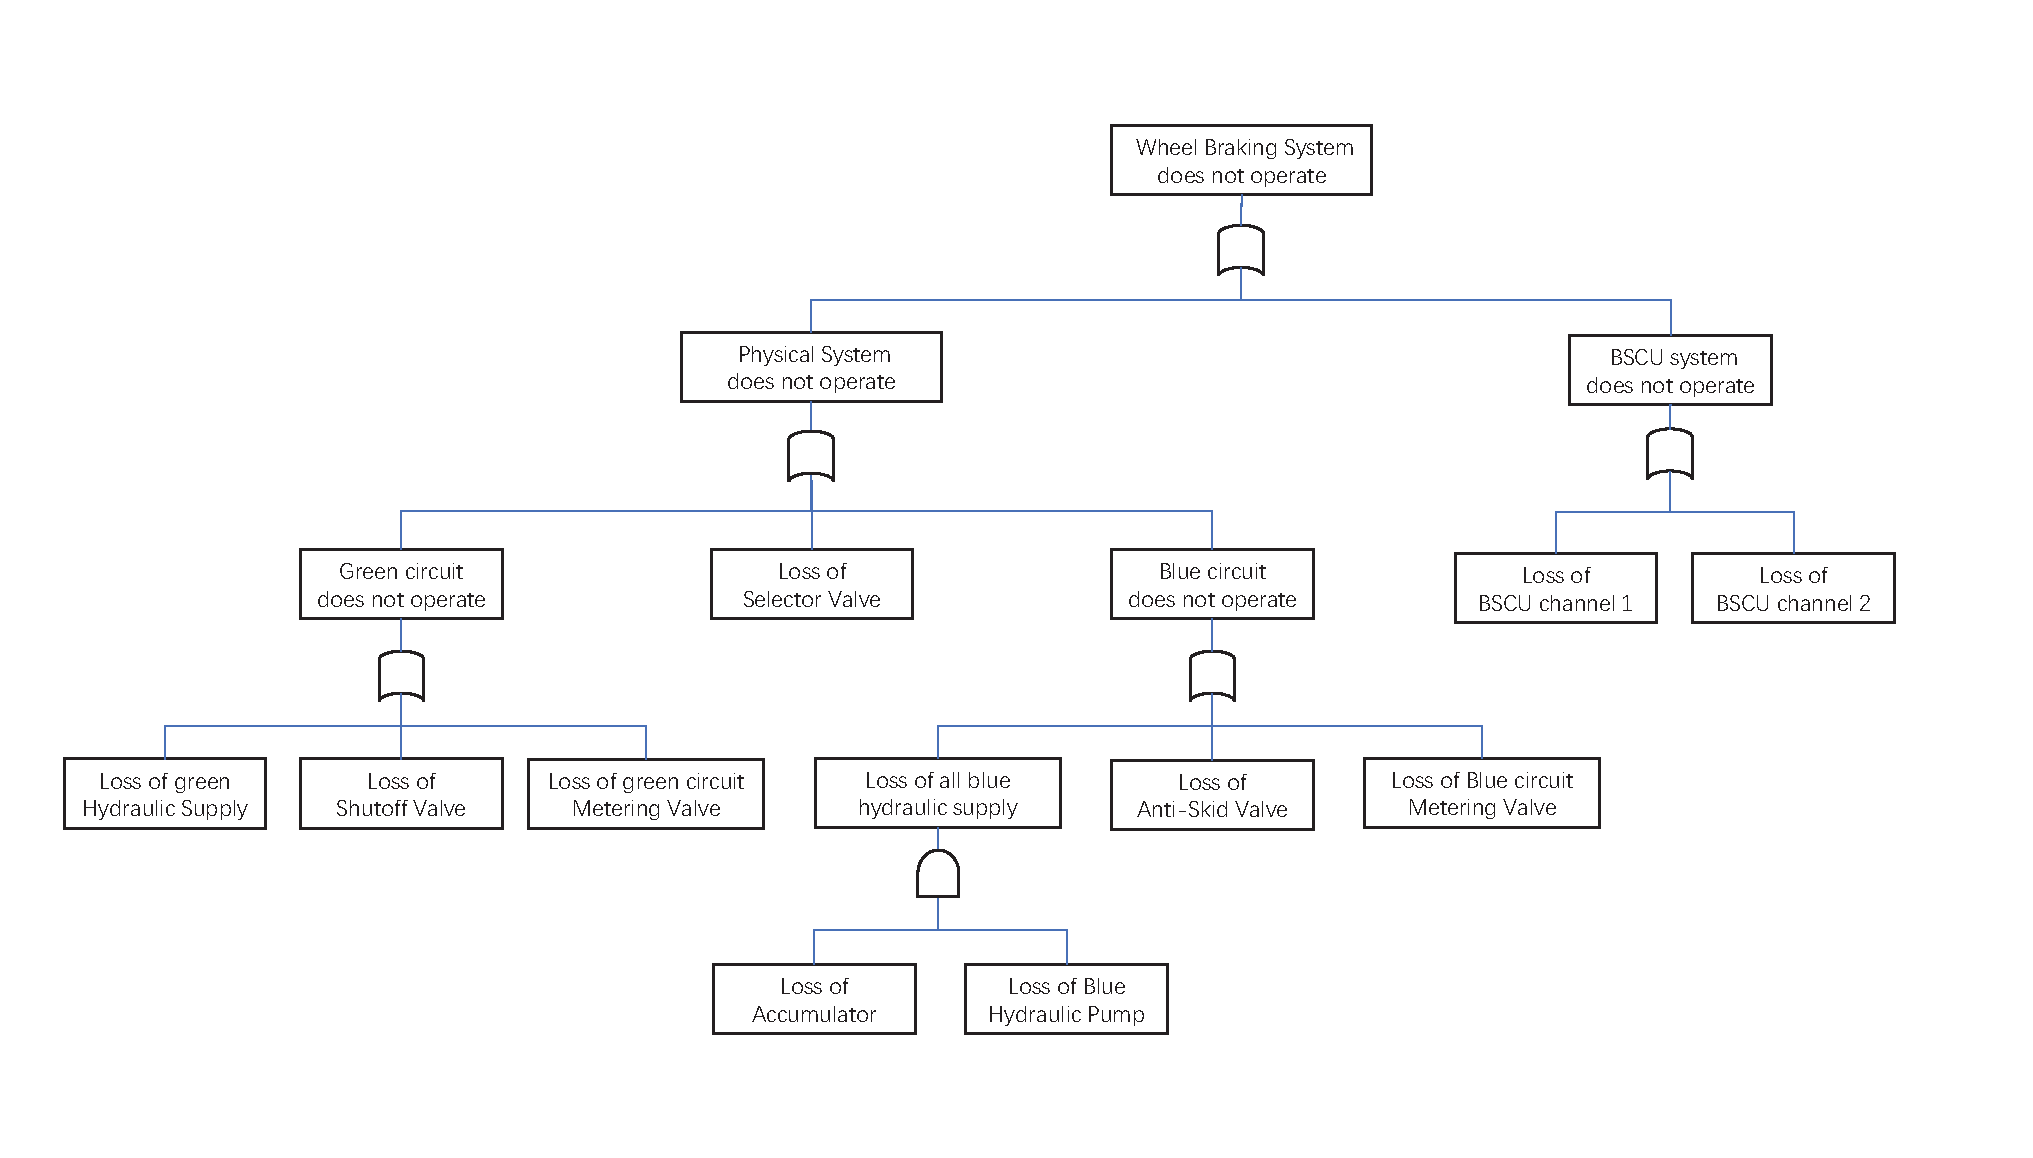
\includegraphics[width=165mm]{figure/fault_tree.eps}}
	\caption{Fault tree for a loss of WBS occurrence under ARCH4}
	\label{WBS_BIP_Nominal}
\end{figure*}

\begin{table}[htbp]
	\caption{Deduced faulty behavior statistics under ARCH4}
	\begin{center}
		\begin{tabular}{|c|c|@{}p{0.002\linewidth}<{\centering}@{}|c|}
			\hline
			\multicolumn{2}{|c|}{}&&{Number of fault(s)}\\
			\hline
			\multirow{3}*{\tabincell{c}{Pumps}}&{Green Hydraulic Pump}&&{1}\\
			\cline{2-4}
			&{Blue Hydraulic Pump}&&{1}\\
			\cline{2-4}
			&{Accumulator}&&{1}\\
			\hline
			\multirow{5}*{\tabincell{c}{Valves}}&{Shutoff Valve}&&{2}\\
			\cline{2-4}
			&{Anti-Skid Valve}&&{2}\\
			\cline{2-4}
			&{Green Meter Valve}&&{2}\\
			\cline{2-4}
			&{Blue Meter Valve}&&{2}\\
			\cline{2-4}
			&{Selector Valve}&&{1}\\
			\hline
			\multirow{2}*{BSCU}&{BSCU channel 1}&&{3}\\
			\cline{2-4}
			&{BSCU channel 2}&&{3}\\
			\hline
		\end{tabular}
		\label{tab1}
	\end{center}
\end{table}

\subsection{Extended WBS Model with faults}
In this section, we give a whole view of modified BIP model which is integrated with fault tree introduced in section \emph{B} using the methodology provided in seciton \emph{A}.

Table 2 shows metrics for the different architectures. The later the design version of the architecture, the greater the scale of the BIP model. ARCH1 shows a large delta with other three architectures. From ARCH2 to ARCH3, there is a differ from the design of the BSCU. For ARCH2, the AIR6110 standard only requires a redundency of BSCU which results in a WBS model including two identical BSCU system. For ARCH3, motivated by trade studies on ARCH2, the strcture is modified from two BSCUs to a BSCU with dual channels. Also, as the result of integration, the extended BIP model with fault behavior presents a larger scale than the nominal BIP model. ARCH3 and ARCH4 show the closest metrics for there is only a little change in the physical system.

The graphical representation of the BIP model can seperate the correct behavior from the faulty behavior to a great extent. This helps us tracing how a single point of failure impacts the system and whether it will cause a top level failure or not. 

The full system implementation can be found at \href{https://github.com/Rosaugo/WBSFaultModelingBIP}{https://github.com/Rosaugo/WBSFaultModelingBIP}. You can find the nominal WBS model or the BIP model extended with the faults described in the fault tree in section \emph{B}.

\begin{table}[htbp]
	\caption{BIP Nominal/Fault Model statistics}
	\begin{center}
\begin{tabular}{|c|c|@{}p{0.002\linewidth}<{\centering}@{}|c|c|c|c|}
	\hline
	\multicolumn{2}{|c|}{}&&{ARCH1}&{ARCH2}&{ARCH3}&{ARCH4}\\
	\hline
	\multirow{2}*{\tabincell{c}{Component\\types}}&{Nominal}&&&&&\\
	\cline{2-7}
	&{Extended}&&&&&\\
	\hline
	\multirow{2}*{\tabincell{c}{Compound\\types}}&{Nominal}&&&&&\\
	\cline{2-7}
	&{Extended}&&&&&\\
	\hline
	\multirow{2}*{Max depth}&{Nominal}&&&&&\\
	\cline{2-7}
	&{Extended}&&&&&\\
	\hline
	\multirow{2}*{Variables}&{Nominal}&&&&&\\
	\cline{2-7}
	&{Extended}&&&&&\\
	\hline
	\multirow{2}*{\tabincell{c}{Internal\\ports}}&{Nominal}&&&&&\\
	\cline{2-7}
	&{Extended}&&&&&\\
	\hline
	\multirow{2}*{\tabincell{c}{External\\ports}}&{Nominal}&&&&&\\
	\cline{2-7}
	&{Extended}&&&&&\\
	\hline
\end{tabular}
		\label{tab1}
	\end{center}
\end{table}

\section{Verification Methodology and Experiments}
In this section, we introduce the application of SBIP tool chains on our WBS BIP model. . Through the experiment results, we demonstrate that our methodology can help system engineers improve the role of specification and promote the iteration of the system architecture.

\subsection{WBS Requirements formalization and decomposition}
The AIR6110 document contains several requirements for the WBS. These can be grouped in two main categories: Requirements corresponding to safety, e.g., \emph{the loss of all wheel braking shall be extremely remote}, and others, e.g., \emph{the WBS shall have at least two hydraulic pressure sources}.

\textcolor{red}{
Giving an explaination of how to translate WBS requirements to LTL specifications and taking one requirement to LTL as an example.
}

\subsection{Experiments and results}
\textcolor{red}{
Briefly introduction.
}

\subsubsection{Probability Estimation}
\ 
\newline 
\textcolor{red}{
\indent Will be texted after further experiments finished.
}

\subsubsection{Parametric exploration}
\ 
\newline 
\textcolor{red}{
	\indent Will be texted after further experiments finished.
}

\section{Conclusions and Future Work}
\textcolor{red}{
	Giving an overview of conclusions and future work here.
}

\section*{Acknowledgment}
\textcolor{red}{
This work was supported by * (check with Prof.Miao). The author wish to thank * (check with everyone)
}

\begin{thebibliography}{00}
\bibitem{b1} G. Eason, B. Noble, and I. N. Sneddon, ``On certain integrals of Lipschitz-Hankel type involving products of Bessel functions,'' Phil. Trans. Roy. Soc. London, vol. A247, pp. 529--551, April 1955.
\end{thebibliography}

\end{document}
